\documentclass[11pt]{article}
\usepackage[margin=1in]{geometry}
\usepackage{booktabs}
\usepackage{graphicx}
\usepackage{float}
\usepackage{caption}
\usepackage{hyperref}
\captionsetup{font=small,labelfont=bf}
\title{Exploratory Data Analysis Report for the GLW CML Dataset}
\author{}
\date{\today}
\begin{document}
\maketitle

\begin{abstract}
This report summarizes data cleaning and exploratory analysis for a chronic myeloid leukemia molecular monitoring dataset. The regenerated public analysis files contain 495 longitudinal molecular observations from 87 coded patients, 275 at-risk interval-survival records, and 87 patient-level records. A total of 68 patients (78.2\%) had an observed deep molecular response (DMR), while 19 patients were censored without observed DMR. The report emphasizes privacy-preserving preprocessing, completeness of modeling variables, longitudinal LOG-MRD trajectories, time to first DMR, cytogenetic response patterns, and data limitations relevant to subsequent joint longitudinal--interval survival modeling.
\end{abstract}

\section{Analysis Objectives}
The EDA had four practical objectives. First, the raw longitudinal and patient-level files were converted into privacy-preserving public analysis tables. Second, complete-case modeling fields were audited so that downstream statistical modeling receives coherent time, outcome, and molecular-measurement variables. Third, cohort-level summaries and high-resolution figures were generated to understand response dynamics and missingness. Fourth, the final LaTeX report, tables, figures, and verification checks were made reproducible from the R scripts in \texttt{04\_Code/R}.

\section{Data Sources and Cleaning}
The raw visit-level file contained 504 rows. After removing records with missing or invalid essential modeling fields, the longitudinal model file contains 495 complete observations. The analysis preserves all direct patient identifiers only in the private key file under \texttt{03\_Data/Processed/private}; public analysis files use coded identifiers of the form \texttt{P0001}.

Treatment time was represented as months since imatinib start. Baseline rows marked as pretreatment measurements were set to time zero; follow-up rows used the treatment-start date and laboratory date when available, with visit-label fallback rules for records that had explicit month labels. DMR was defined as \texttt{log\_mrd <= -4.5}; complete molecular response (CMR) was defined as \texttt{log\_mrd <= -5.0}.

\begin{table}[!htbp]
\centering
\caption{Data cleaning audit and generated analysis datasets.}
\label{tab:cleaning-audit}
\resizebox{\linewidth}{!}{%
\begin{tabular}{lr}
\toprule
Cleaning step & Count \\
\midrule
raw\_longitudinal\_rows & 504 \\
raw\_longitudinal\_patients &  89 \\
dropped\_missing\_or\_invalid\_core\_fields &   9 \\
model\_ready\_longitudinal\_rows & 495 \\
model\_ready\_longitudinal\_patients &  87 \\
raw\_patient\_table\_rows &  87 \\
usable\_patient\_covariate\_rows &  71 \\
patient\_level\_analysis\_rows &  87 \\
complete\_core\_covariate\_rows &  62 \\
interval\_survival\_rows & 275 \\
dmr\_event\_patients &  68 \\
censored\_patients &  19 \\
\bottomrule
\end{tabular}
}%
\end{table}

\begin{table}[!htbp]
\centering
\caption{Missing or invalid fields in the raw longitudinal file.}
\label{tab:missingness}
\resizebox{\linewidth}{!}{%
\begin{tabular}{lr}
\toprule
Variable & Missing or invalid rows \\
\midrule
ratio & 9 \\
log\_mrd & 9 \\
lab\_date & 4 \\
sample\_type & 4 \\
abl\_copy & 4 \\
IS & 3 \\
patient\_name & 0 \\
bcr\_abl\_copy & 0 \\
t\_months & 0 \\
\bottomrule
\end{tabular}
}%
\end{table}


\section{Cohort Description}
The patient-level analysis table contains 87 coded patients. Baseline covariates are available for a subset: 62 patients (71.3\%) have complete core covariates for age, treatment duration, baseline Philadelphia chromosome percentage, and sex. Among patients with non-missing age, the mean age was 44.6 (SD 15.5; n=62) years. Male patients accounted for 38 (61.3\%; n=62) of those with recorded sex.

Follow-up was heterogeneous, with median follow-up of 39.0 [15.8, 65.8] months and a median of 5 [4, 7] visits per patient. Patients with observed DMR had longer median observed follow-up (46.5 [23.1, 71.7] months) than censored patients (13.0 [10.8, 24.1] months), which is expected because longer observation creates more opportunity to document response.

\input{../06_Tables/table_01_baseline_characteristics.tex}

\section{Longitudinal Molecular Patterns}
The longitudinal file contains 495 complete molecular measurements. Baseline or first-observed LOG-MRD had median -1.4 [-2.8, -1.0], while the last observed LOG-MRD per patient had median -5.0 [-5.0, -1.4]. Across all visits, 239 observations (48.3\%) met the DMR threshold and 239 observations (48.3\%) met the CMR threshold.

Figure~\ref{fig:log-mrd-trajectories} shows strong early decline in the smoothed LOG-MRD trend, followed by a flatter low-level trajectory. Individual trajectories vary substantially, supporting the need for patient-specific random effects in downstream longitudinal modeling.

\begin{table}[!htbp]
\centering
\caption{Longitudinal molecular monitoring summaries by follow-up window.}
\label{tab:longitudinal-time}
\resizebox{\linewidth}{!}{%
\begin{tabular}{lrrrrrr}
\toprule
Window\_months & Observations & Patients & BM\_samples & LOG\_MRD & DMR & CMR \\
\midrule
0-3 &  67 & 55 & 67 (100.0\%); n=67 & -1.2 [-1.6, -0.8]; n=67 & 2 (3.0\%); n=67 & 2 (3.0\%); n=67 \\
$>$3-6 &  36 & 34 & 36 (100.0\%); n=36 & -2.0 [-3.5, -1.1]; n=36 & 8 (22.2\%); n=36 & 8 (22.2\%); n=36 \\
$>$6-12 &  79 & 59 & 79 (100.0\%); n=79 & -2.7 [-5.0, -1.6]; n=79 & 26 (32.9\%); n=79 & 26 (32.9\%); n=79 \\
$>$12-24 &  95 & 59 & 92 (96.8\%); n=95 & -5.0 [-5.0, -2.4]; n=95 & 51 (53.7\%); n=95 & 51 (53.7\%); n=95 \\
$>$24-60 & 135 & 53 & 134 (99.3\%); n=135 & -5.0 [-5.0, -2.4]; n=135 & 90 (66.7\%); n=135 & 90 (66.7\%); n=135 \\
$>$60 &  83 & 26 & 83 (100.0\%); n=83 & -5.0 [-5.0, -4.5]; n=83 & 62 (74.7\%); n=83 & 62 (74.7\%); n=83 \\
\bottomrule
\end{tabular}
}%
\end{table}


\begin{figure}[!htbp]
\centering
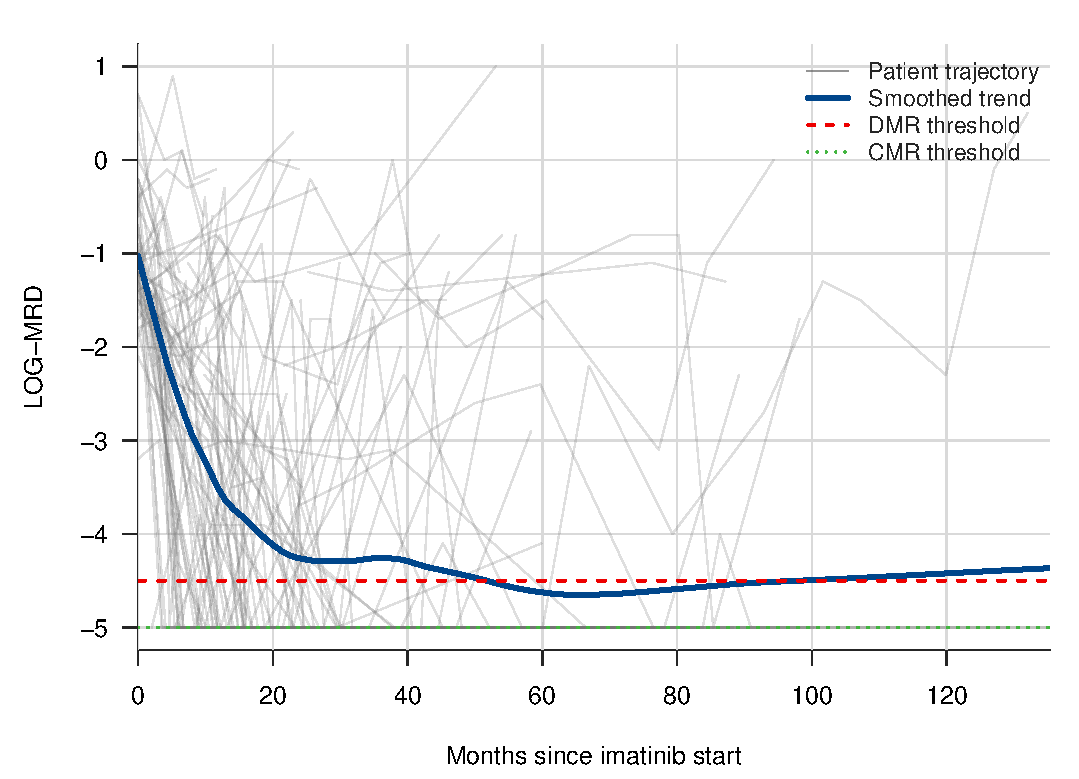
\includegraphics[width=0.92\linewidth]{../05_Figures/figure_01_log_mrd_trajectories.pdf}
\caption{Patient-level LOG-MRD trajectories with smoothed population trend and DMR/CMR thresholds.}
\label{fig:log-mrd-trajectories}
\end{figure}

\section{Time to Deep Molecular Response}
DMR was observed for 68 of 87 patients (78.2\%). Among event patients, the observed time to first DMR had median 14.8 [9.0, 27.0] months. The interval-survival table contains 275 at-risk intervals and encodes only the first interval ending in observed DMR for each patient.

The Kaplan--Meier curve in Figure~\ref{fig:time-to-dmr} shows a rapid early decrease in the probability of remaining without observed DMR, followed by a long tail of delayed or unobserved responders. Because DMR is observed only at monitoring visits, interval-based survival modeling is more appropriate than treating event times as exact.

\begin{figure}[!htbp]
\centering
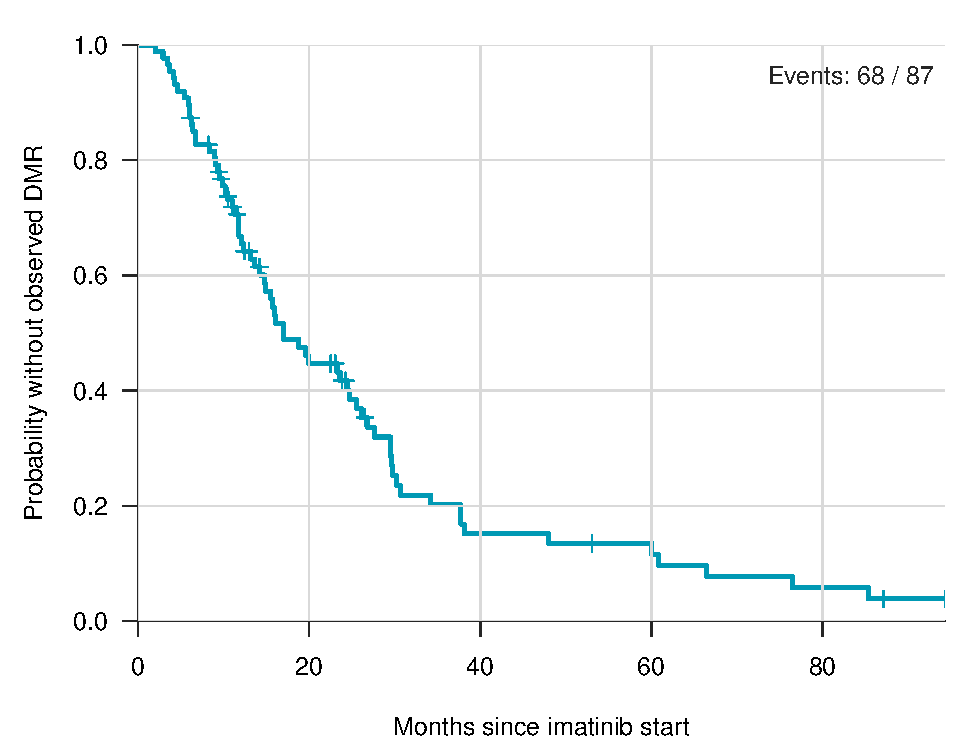
\includegraphics[width=0.78\linewidth]{../05_Figures/figure_02_time_to_dmr_km.pdf}
\caption{Kaplan--Meier curve for time until first observed DMR. Censoring marks indicate patients without observed DMR by last follow-up.}
\label{fig:time-to-dmr}
\end{figure}

\section{Cytogenetic Response}
Cytogenetic measurements were most complete at baseline (n=62) and became sparser over later landmarks (3 months n=44, 6 months n=52, 12 months n=59, 18 months n=58, 24 months n=49). Median Philadelphia chromosome positivity was 100.0 [100.0, 100.0] at baseline and 0.0 [0.0, 0.0] at 12 months among available records.

Figure~\ref{fig:cytogenetic-response} suggests a marked reduction in Philadelphia chromosome positivity after treatment initiation, though later landmark summaries should be interpreted cautiously because the available sample size decreases and follow-up schedules are irregular.

\begin{figure}[!htbp]
\centering
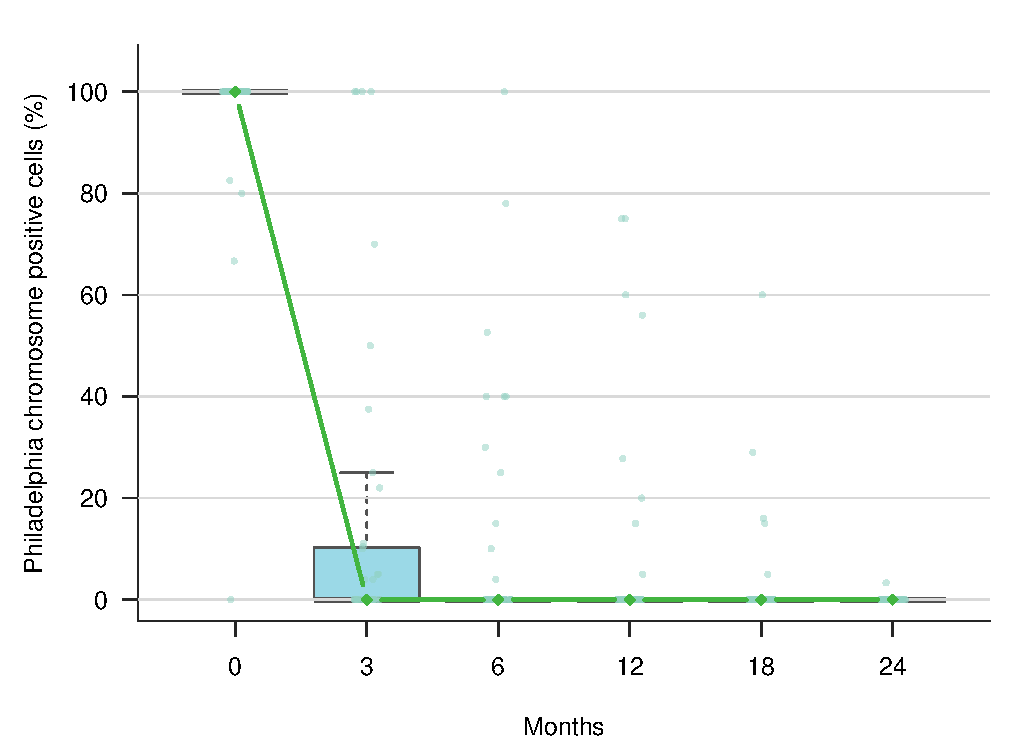
\includegraphics[width=0.82\linewidth]{../05_Figures/figure_03_cytogenetic_response.pdf}
\caption{Distribution of Philadelphia chromosome positive cells over follow-up among patients with available cytogenetic data.}
\label{fig:cytogenetic-response}
\end{figure}

\section{Visit Schedule and Missingness}
The monitoring schedule was irregular. Visit times had median 20.7 [7.1, 45.7] months from treatment start, and positive inter-visit gaps had median 6.5 [4.1, 11.4] months. The most common missing or invalid raw longitudinal fields were ratio (9 rows), log\_mrd (9 rows), lab\_date (4 rows).

Figure~\ref{fig:visit-timing} shows that many measurements occurred early after treatment initiation, with progressively fewer late measurements. Figure~\ref{fig:raw-missingness} shows that essential molecular fields were mostly complete, but missing LOG-MRD, ratio, laboratory date, specimen type, and ABL copy values drove most exclusions.

\begin{figure}[!htbp]
\centering
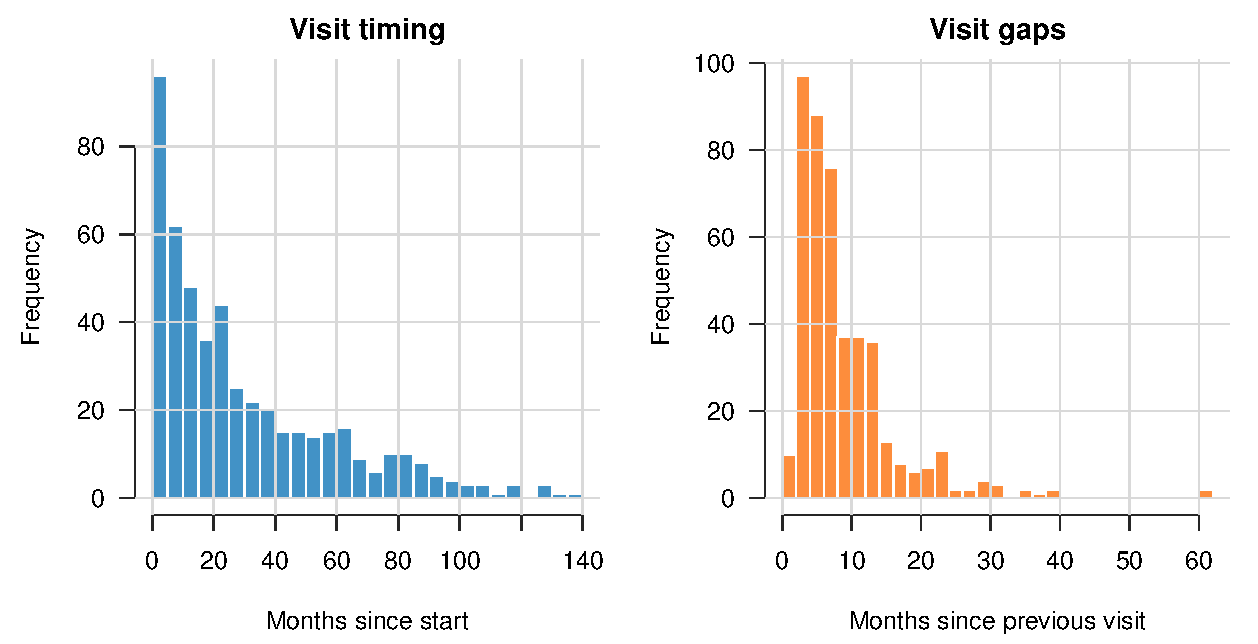
\includegraphics[width=0.95\linewidth]{../05_Figures/figure_04_visit_timing_and_gaps.pdf}
\caption{Monitoring time distribution and inter-visit gap distribution in the cleaned longitudinal data.}
\label{fig:visit-timing}
\end{figure}

\begin{figure}[!htbp]
\centering
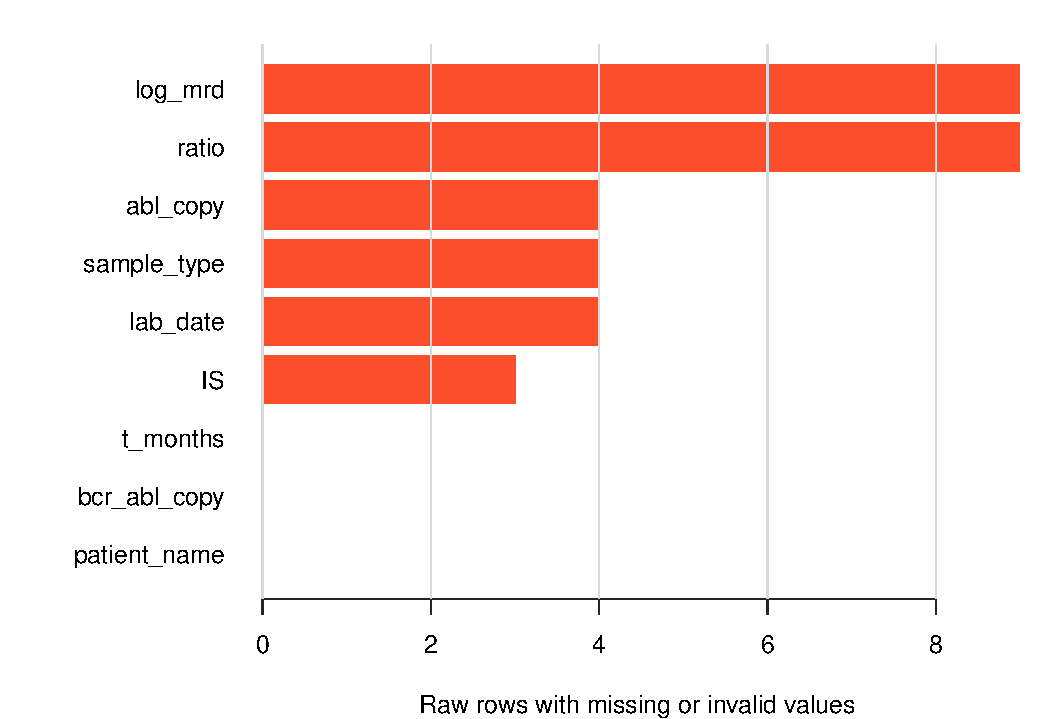
\includegraphics[width=0.78\linewidth]{../05_Figures/figure_05_raw_missingness.pdf}
\caption{Raw longitudinal missingness in essential modeling fields.}
\label{fig:raw-missingness}
\end{figure}

\section{Modeling Implications}
\begin{itemize}
\item The cleaned longitudinal data are suitable for modeling LOG-MRD trajectories with patient-specific intercepts and slopes.
\item The response endpoint should be handled as interval observed because DMR is detected at irregular monitoring visits rather than at a continuous exact event time.
\item Baseline covariate adjustment should be treated as secondary or sensitivity analysis because complete core covariates are available for only a subset of patients.
\item The public modeling datasets are privacy preserving; direct patient names are excluded from public outputs and retained only in the private linkage file.
\end{itemize}

\section{Generated Reproducible Outputs}
The EDA pipeline generated the public model-ready CSV files under \texttt{03\_Data/Processed}, high-resolution 600 dpi PNG figures and vector PDF figures under \texttt{05\_Figures}, table CSV and LaTeX fragments under \texttt{06\_Tables}, and this compiled report under \texttt{02\_LaTeX}. The driver script \texttt{04\_Code/R/run\_all.R} rebuilds the complete workflow and runs verification checks for completeness, privacy, nonempty artifacts, and interval-event consistency.

\end{document}
